%!TEX program = pdflatex
\documentclass[UTF8]{ctexart}
\usepackage{amsmath}
\usepackage{booktabs}
\usepackage{lmodern}
\usepackage{geometry}
\usepackage{graphicx}
\usepackage[english]{babel}
\usepackage{float}
\ctexset{section={format={\Large\bfseries}}}
\geometry{a4paper,scale=0.8, centering}
\pagenumbering{arabic}
\graphicspath{{./image/}}

\title{\vspace{-1cm}CQF Exam Three\\Decision Trees and Ensembles}
\author{Kai Zheng}
\date{June 07, 2022}
\begin{document}
\maketitle

\section*{Introduction \& Preparetion}

\subsection*{1. Dataset}

For this experiment, we choose BTCUSDT Futures Kline Data (hourly) as the target form. We download data from 2020-01-01 to 2022-04-30\footnote{www.binance.com}. The total row count is 20279 and no non-null data. This dataset is almost eaqued to 5-year period kline (daily) data.

The following figure shows the trend in the first half and the shock in the second half. More information about dataset can be asscessed by notebook\footnote{'1. data, factors and pca.ipynb'}

\begin{figure}[htbp]
	\centerline{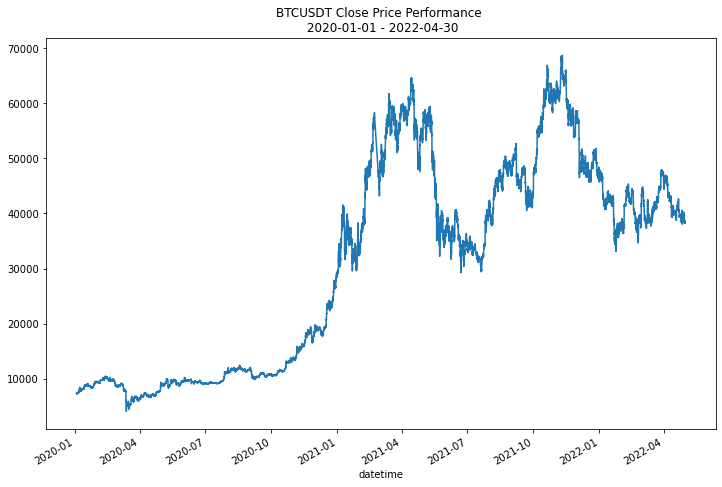
\includegraphics[width=0.80\textwidth]{close_price.png}}
	\caption{BTCUSDT Close Price Performance}
\end{figure}

\subsection*{2. Factor Engineering}

The factors are designed following by the requirements of the exam. The factor zoo includes 18 factors, such as 'O-C', 'H-L', 'PR5', 'PR10', 'PR20', 'PR30', 'PR60', 'MOM5', 'MOM10', 'MOM20', MOM30', 'MOM60', 'SMA5', 'SMA10', 'SMA20', 'SMA30', 'SMA60', and 'EMA'. 'Sign' is designed as the label.

\begin{figure}[htbp]
	\centerline{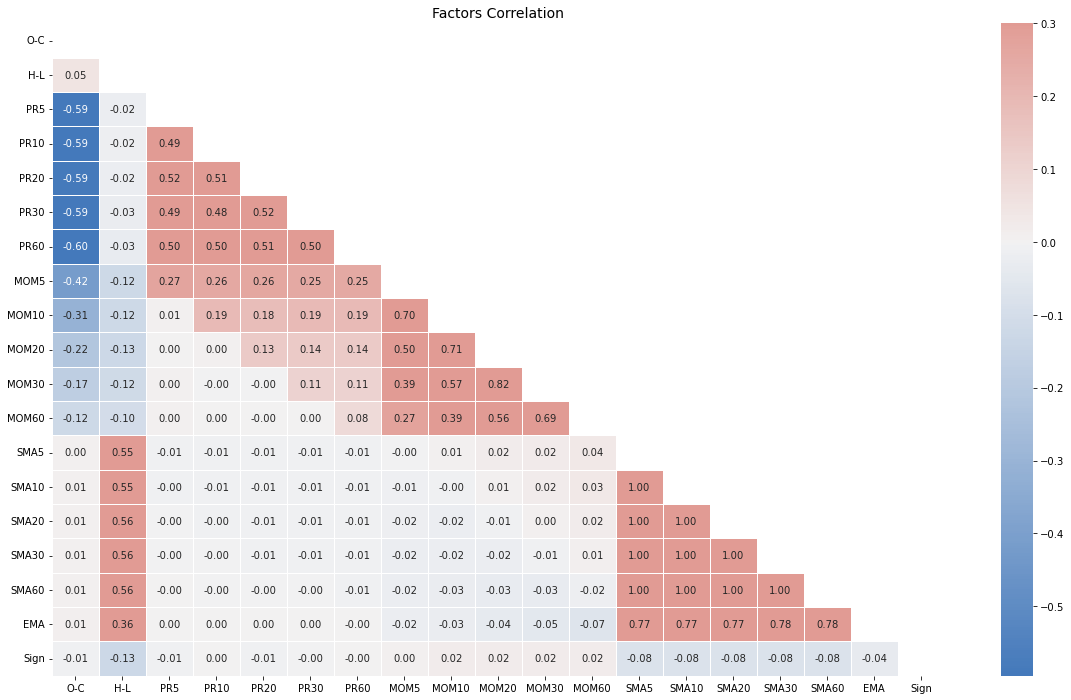
\includegraphics[width=0.95\textwidth]{factors_corr.png}}
	\caption{Factors Correlation}
\end{figure}

\subsection*{3. PCA}

PCA is used to decompose a multivariate dataset in a set of successive orthogonal components that explain a maximum amount of the variance\footnote{https://scikit-learn.org/stable/modules/decomposition.html\#principal-component-analysis-pca}. The original 18 factors were reduced to 8 factors by PCA.

\begin{table}[htbp]
	\centering
	\begin{tabular}{lrrrr}
		\toprule
		                 & MSE    & RMSE   & R2Train & R2Test \\
		\midrule
		Original Factors & 0.4946 & 0.7032 & 1.0000  & 0.5054 \\
		PCA Factors      & 0.4951 & 0.7036 & 1.0000  & 0.5049 \\
		\bottomrule
	\end{tabular}
	\setlength{\abovecaptionskip}{0.3cm}
	\setlength{\belowcaptionskip}{0cm}

	\caption{Original Factors vs. PCA Factors}
\end{table}

Comparing the score of original factors with PCA factors, we found that MSE increased from 0.4946 to 0.4951, and R2Test decresed from 0.5054 to 0.5049. Considering the reduced amount of data and computation, the results are acceptable with less MSE and R2 Score.

\subsection*{4. How to categorise small near-zero returns}

How to categorise returns can be described as:

\begin{equation}
	y_t= \left\{
	\begin{aligned}
		+1 & , if\ p_{t+1} > ratio * p_t \\
		0  & , if\ p_{t+1}\ \ otherwise  \\
	\end{aligned}
	\right\}
\end{equation}

We notice that MSE and $R^2$ score is difference when the ratio changes, so the experiment will focus on the relation between ratio and directors. We set the sign ratio from 0.9 to 1.15, increasing by 0.0005 each step. Several indicators were counted in the experement. From Figure 3, we can find that when ratio eaques 1.0, the positive almost eaques to the negative count.

\begin{figure}[H]
	\centerline{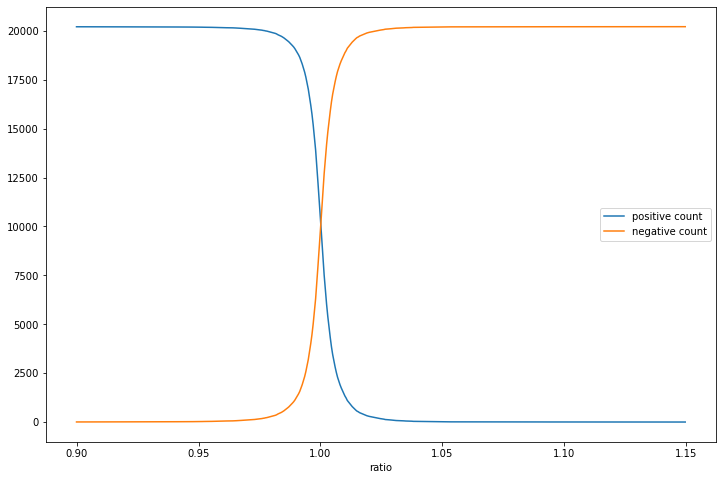
\includegraphics[width=0.70\textwidth]{sign_count.png}}
	\caption{Sign Count}
\end{figure}

\begin{figure}[H]
	\centerline{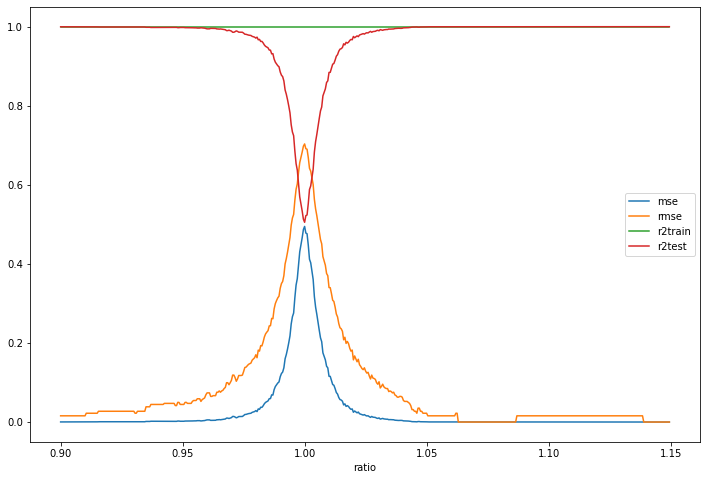
\includegraphics[width=0.70\textwidth]{sign_ratio.png}}
	\caption{Indicators}
\end{figure}

From the Figure 4, we can find that when ratio eaques 1.0, the mse is the higest and the score is the lowest, and when decrease or increase ratio, the mse decreses and the score increases. If the ratio is smaller than 0.95 or bigger than 1.05, overfitting happens.

\begin{table}[htbp]
	\centering
	\begin{tabular}{rrrrrrr}
		\toprule
		Ratio  & MSE    & RMSE   & R2Train & R2Test & Positive Count & Negative Count \\
		\midrule
		0.9950 & 0.2663 & 0.5161 & 1.0000  & 0.7337 & 17019.0000     & 3198.0000      \\
		0.9995 & 0.4869 & 0.6978 & 1.0000  & 0.5131 & 11295.0000     & 8922.0000      \\
		1.0000 & 0.4948 & 0.7034 & 1.0000  & 0.5052 & 10346.0000     & 9871.0000      \\
		\cline{1-7}
		1.0005 & 0.4780 & 0.6914 & 1.0000  & 0.5220 & 9385.0000      & 10832.0000     \\
		1.0050 & 0.2725 & 0.5220 & 1.0000  & 0.7275 & 3447.0000      & 16770.0000     \\
		\bottomrule
	\end{tabular}
	\setlength{\abovecaptionskip}{0.3cm}
	\setlength{\belowcaptionskip}{0cm}

	\caption{Sign Ratio Performance Comparison table}
\end{table}

Considering the balance of the sign distribution, 1.0 ratio is the best choice for the experiment. If the ratio is changed to be unbalanced, the indicators will be biased to one direction.

\section*{Question 1. Theory Task}

\subsection*{1. Mathematically specify three types of Loss Function}

\subsubsection*{a. Information Gain}

ID3 (Iterative Dichotomiser 3) was developed in 1986 by Ross Quinlan. The algorithm creates a multiway tree, finding for each node (i.e. in a greedy manner) the categorical feature that will yield the largest information gain for categorical targets. Trees are grown to their maximum size and then a pruning step is usually applied to improve the ability of the tree to generalize to unseen data.

\begin{equation}
	Ent(D) = -\sum_{k=1}^{|y|} p_k \log_2 p_k
\end{equation}

\begin{equation}
	Gain(D, a) = Ent(D) - \sum_{v=1}^{V} \frac{|D^v|}{|D|} Ent(D^v)
\end{equation}

\subsubsection*{b. Gain Ration}

C4.5 is the successor to ID3 and removed the restriction that features must be categorical by dynamically defining a discrete attribute (based on numerical variables) that partitions the continuous attribute value into a discrete set of intervals. C4.5 converts the trained trees (i.e. the output of the ID3 algorithm) into sets of if-then rules.

\begin{equation}
	Gain(D, a) = Ent(D) - \sum_{v=1}^{V} \frac{|D^v|}{|D|} Ent(D^v)
\end{equation}

\begin{equation}
	Gain_Ratio(D, a) = \frac{Gain(D, a)}{IV(a)}
\end{equation}

\subsubsection*{c. Gini Index}

CART (Classification and Regression Trees) is very similar to C4.5, but it differs in that it supports numerical target variables (regression) and does not compute rule sets. CART constructs binary trees using the feature and threshold that yield the largest information gain at each node.

\begin{equation}
	\begin{aligned}
		Gini(D) & = \sum_{k=1}^{y} \sum_{k'\neq k} p_k p_{k'} \\
		        & = 1 - \sum_{k=1}^{y} p_k^2
	\end{aligned}
\end{equation}

\begin{equation}
	Gini_index(D, a) = \sum_{v=1}^{V} \frac{|D^v|}{|D|} Gini(D^v)
\end{equation}

\subsection*{2. Which data transformation can prepare the data for linear separation?}

In order to do the experiment,   We choose LogisticRegression as the linear model and 5 common scalers: StandardScaler, MinMaxScaler, MaxAbsScaler, QuantileTransformer, and PowerTransformer to test 4 indicators: MSE, RMSE, R2Train, and R2Test.

\begin{table}[htbp]
	\centering

	\begin{tabular}{lrrrr}
		\toprule
		Scaler              & MSE    & RMSE   & R2Train & R2Test \\
		\midrule
		StandardScaler      & 0.4691 & 0.6849 & 0.5368  & 0.5309 \\
		MinMaxScaler        & 0.4718 & 0.6869 & 0.5360  & 0.5282 \\
		MaxAbsScaler        & 0.4691 & 0.6849 & 0.5348  & 0.5309 \\
		QuantileTransformer & 0.4594 & 0.6778 & 0.5423  & 0.5406 \\
		PowerTransformer    & 0.4676 & 0.6838 & 0.5360  & 0.5324 \\
		\bottomrule
	\end{tabular}

	\setlength{\abovecaptionskip}{0.3cm}
	\setlength{\belowcaptionskip}{0cm}

	\caption{Transformation Test Result}
\end{table}

From table 3, we can find that MinMaxScaler has the lowest MSE and RMSE scores which mean the lowest amount of error, and has the highest R2Train and R2Test scores which indicate more variability is explained. So it can be concluded that MinMaxScaler is the best scaler for this experiment.

\section*{Question 2. Implementation Tasks for Models Type}

\subsection*{1. Vary hyperparameters RandomizedSearchCV and GridSearchCV}

The grid search provided by GridSearchCV exhaustively generates candidates from a grid of parameter values specified with the param\_grid parameter\footnote{https://scikit-learn.org/stable/modules/grid\_search.html\#exhaustive-grid-search}. RandomizedSearchCV implements a randomized search over parameters, where each setting is sampled from a distribution over possible parameter values\footnote{https://scikit-learn.org/stable/modules/grid\_search.html\#randomized-parameter-optimization}.

The parameters of search can be split into 'criterion', 'max\_depth', 'max\_features', 'min\_samples\_leaf' and 'min\_samples\_split'. In this question, we use 'gini' and 'entropy' as the scope of criterion, number range from 1 to 10 as the scope of other parameters.

\begin{table}[htbp]
	\centering
	\begin{tabular}{lll}
		\toprule
		Hyperparameter      & GridSearchCV & RandomizedSearchCV \\
		\midrule
		criterion           & gini         & gini               \\
		max\_depth          & 1            & 1                  \\
		max\_features       & 6            & 7                  \\
		min\_samples\_leaf  & 1            & 6                  \\
		min\_samples\_split & 2            & 7                  \\
		\cline{1-3}
		best\_score\_       & 0.536974     & 0.536974           \\
		\bottomrule
	\end{tabular}
	\setlength{\abovecaptionskip}{0.3cm}
	\setlength{\belowcaptionskip}{0cm}

	\caption{Hyperparameters Result}
\end{table}

Table 3 is the result of GridSearchCV and RandomizedSearchCV. We can see that there are little differences between them and the best scores are the same.

\begin{table}[htbp]
	\centering
	\begin{tabular}{lrrrr}
		\toprule
		Search Type        & MSE    & RMSE   & R2Train & R2Test \\
		\midrule
		No Hyperparameters & 0.4946 & 0.7032 & 1.0000  & 0.5054 \\
		GridSearchCV       & 0.4711 & 0.6863 & 0.5397  & 0.5289 \\
		RandomizedSearchCV & 0.4763 & 0.6901 & 0.5355  & 0.5237 \\
		\bottomrule
	\end{tabular}

	\setlength{\abovecaptionskip}{0.3cm}
	\setlength{\belowcaptionskip}{0cm}

	\caption{Hyperparameters Score}
\end{table}

From table 4, GridSearchCV and RandomizedSearchCV provide better parameters for the model. The difference between GridSearchCV and RandomizedSearchCV is very small. We notice that the cost time of GridSearchCV is 3m 50s, much longer than RandomizedSearchCV 1s. So, if the run time is too long,  RandomizedSearchCV is another better solusion.

\subsection*{2. Formulate up to four principles of trees pruning}

Decision-tree learners can create over-complex trees that do not generalize the data well. This is called overfitting. Pruning is the process that helps in preventing the overfitting of the training data. It is divided into two types:

\subsubsection*{1. Pre-Pruning}

Pre pruning is nothing but stoping the growth of decision tree on an early stage. For that we can limit the growth of trees by setting constrains. We can limit parameters like max\_depth, min\_samples etc.

\subsubsection*{2. Post-Pruning}

\subsubsection*{a. Reduced Error Pruning}

Reduced error pruning can reduce overfitting, but it also reduces the amount of data available for training. C4.5 uses a pruning technique based on statistical confidence estimates\footnote{http://www.cs.bc.edu/~alvarez/ML/statPruning.html}. This technique has the advantage that it allows all of the available labeled data to be used for training. The heart of the statistical pruning technique is the calculation of a confidence interval for the error rate.

\begin{equation}
	p = f \pm z * \sqrt{\frac{f * (1 - f)}{N} }
\end{equation}

Here, f, p, and N are as described above. z is a factor that depends on the desired level of confidence.

In order to decide whether to replace a near-leaf node and its child leaves by a single leaf node, C4.5 compares the upper limits of the error confidence intervals for the two trees. For the unpruned tree, the upper error estimate is calculated as a weighted average over its child leaves. Whichever tree has a lower estimated upper limit on the error rate "wins" and is selected.

\subsubsection*{b. Minimal Cost-Complexity Pruning}

Minimal cost-complexity pruning is an algorithm used to prune a tree to avoid over-fitting\footnote{https://scikit-learn.org/stable/modules/tree.html\#minimal-cost-complexity-pruning}. This algorithm is parameterized by $\alpha > 0$ known as the complexity parameter. The complexity parameter is used to define the cost-complexity measure, $R_\alpha (T)$ of a given tree $T$:

\begin{equation}
	R_\alpha(T) = R(T) + \alpha |\tilde{T}|
\end{equation}

where $|\tilde{T}|$ is the number of terminal nodes in $T$ and $R(T)$ is traditionally defined as the total misclassification rate of the terminal nodes. A non-terminal node with the smallest value of $\alpha_{eff}$ is the weakest link and will be pruned. This process stops when the pruned tree's minimal $\alpha_{eff}$ is greater than the $ccp_alpha$ parameter.

\subsubsection*{c. Pessimistic Error Pruning}

Niblett and Brotko came it up in 1991 (Cestnik and Bratko 1991). The process is bottom-up which seeks a single tree that minimizes the expected error rate on new samples\footnote{https://scientistcafe.com/ids/tree-pruning}. If we prune a splitting point $t$, all the samples under $t$ will be classified as from one category, say category $c$. If we prune the subtree, the expected error rate is:

\begin{equation}
	\begin{aligned}
		E(t) = \frac{n_t - n_{t,c} + k - 1}{n_t + k}
	\end{aligned}
\end{equation}
where
\begin{equation}\nonumber
	\begin{aligned}
		 & k       = number of categories                               \\
		 & n_t     = sample size under node t                           \\
		 & n_{t,c} = number of sample under t that belong to category c \\
	\end{aligned}
\end{equation}

Based on the above definition, the pruning process is (F. Espoito and Semeraro 1997):

\begin{itemize}
	\item Calculate the expected error rate for each non-leave node if that subtree is pruned
	\item Calculate the expected error rate for each non-leave node if that subtree is not pruned
	\item If pruning the node leads to higher expected rate, then keep the subtree; otherwise, prune it.
\end{itemize}

We use hyperparameters from last section as Pre Pruning and use 'ccp\_alpha' as Post Pruning\footnote{https://scikit-learn.org/stable/modules/tree.html\#minimal-cost-complexity-pruning}. The experiment shows that 'ccp\_alpha' always eaques 0 after Pre Pruning.

\begin{table}[htbp]
	\centering
	\begin{tabular}{lrrrr}
		\toprule
		                              & MSE        & RMSE       & R2Train    & R2Test     \\
		\midrule
		Original Factors              & 0.49455984 & 0.70324949 & 1.00000000 & 0.50544016 \\
		Original Factors with Pruning & 0.47106825 & 0.68634412 & 0.53972671 & 0.52893175 \\
		PCA Factors                   & 0.49505440 & 0.70360102 & 1.00000000 & 0.50494560 \\
		PCA Factors with Pruning      & 0.49332344 & 0.70236988 & 0.52241390 & 0.50667656 \\
		\bottomrule
	\end{tabular}
	\setlength{\abovecaptionskip}{0.3cm}
	\setlength{\belowcaptionskip}{0cm}

	\caption{Pruning Test Result}
\end{table}

From the result table, Pruning works. After Pruning, MSE of Original Factors decreases from 0.49 to 0.47 and MSE of PCA Factors decreases from 0.4950 to 0.4933. R2Test Score of Original Factors increases from 0.50 to 0.53 and R2Test Score of PCA Factors increases from 0.5049 to 0.5067. Obviously, Pruning plays a greater role in big data sets. For more infomation, please refer to '5. pruning.ipynb'

\subsubsection*{3. Provide attribution to splits}

We use PCA Factors and he proportions of test data are: 0.1, 0.2, 0.3, 0.4, 0.5. The experiment will calculate MSE and R2 Scroe by using the different proportions.

\begin{table}[htbp]
	\centering
	\begin{tabular}{rrrrr}
		\toprule
		test ratio & mse    & rmse   & r2train & r2test \\
		\midrule
		0.1000     & 0.4654 & 0.6822 & 0.5195  & 0.5346 \\
		0.2000     & 0.4933 & 0.7024 & 0.5224  & 0.5067 \\
		0.3000     & 0.4906 & 0.7004 & 0.5235  & 0.5094 \\
		0.4000     & 0.4814 & 0.6938 & 0.5226  & 0.5186 \\
		0.5000     & 0.4871 & 0.6979 & 0.5255  & 0.5129 \\
		\bottomrule
	\end{tabular}
	\setlength{\abovecaptionskip}{0.3cm}
	\setlength{\belowcaptionskip}{0cm}

	\caption{Splits Test Result}
\end{table}

\begin{figure}[H]
	\centerline{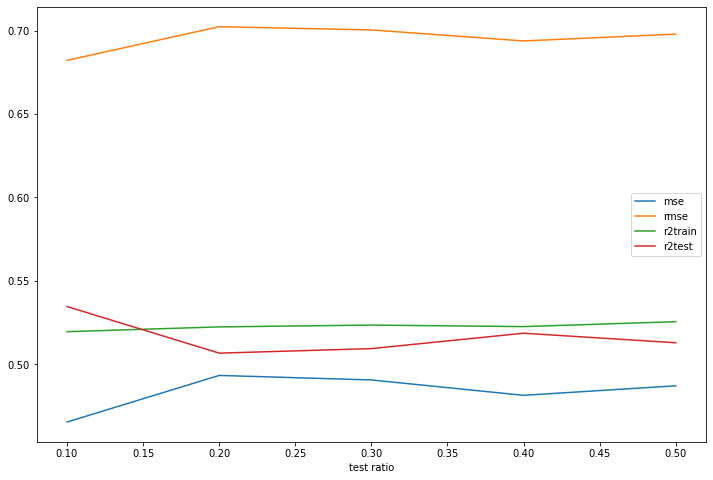
\includegraphics[width=0.70\textwidth]{splits.png}}
	\caption{Splits Test Result}
\end{figure}

The result shows that even the test ratio is from 10\% to 50\%, MSE and R2 Score only changes by 3\% at most. So we can draw a conclusion that the splits are insensible in this experiment. For more infomation, please refer to '6. splits.ipynb'.

\subsubsection*{4. Decision boundaries, ROC and Confusion Matrix}

In this section, we focus on the issues for prediction quality of tree models. During the hyperparameters tuning, we know that the following issues will greatly affect the results\footnote{https://www.educba.com/decision-tree-hyperparameters/}.

\begin{itemize}
	\item \textbf{max\_depth}            \\
	      'max\_depth' is suggested the maximum depth that we allow the tree to grow to. The deeper you allow, the more complex our model will become. If we increase the max\_depth value, training error will always go down but let us consider a case for testing error; if we set the max\_depth too high, then without capturing the useful patterns, the decision tree might simply overfit the training data, this will cause the testing error to increase, but if we set the value of it to too low that is also not good then the decision tree might be having little flexibility to capture the patterns and interaction in the training data.

	\item \textbf{min\_samples\_split}   \\
	      'min\_sample\_split' specifies the minimum number of samples required to splits an internal code.

	\item \textbf{min\_samples\_leaf}    \\
	      'min\_samples\_leaf' is the minimum number of samples that we can specify to term a given node as a leaf node so that we do not want to split it further.

	\item \textbf{max\_features}         \\
	      'max\_features' represents the number of features.

\end{itemize}

This figure shows the decision boundaries with hyperparameters from last section (max\_depth=1, max\_features=6, min\_samples\_leaf=1, min\_samples\_split=2).

\begin{figure}[H]
	\centerline{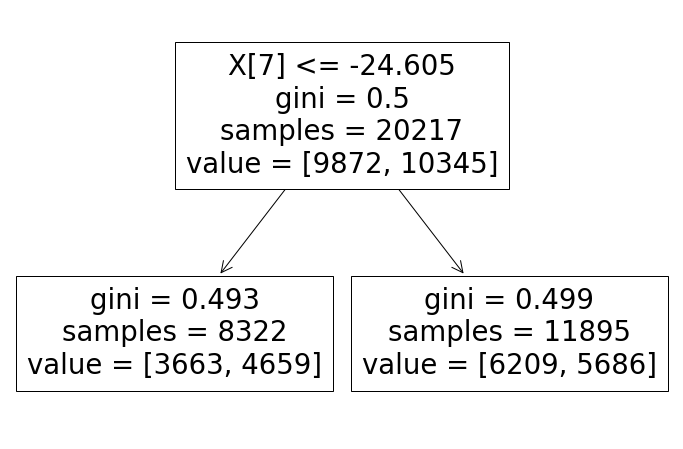
\includegraphics[width=0.70\textwidth]{decision_boundaries.png}}
	\caption{Decision Boundaries}
\end{figure}

The experiment is divided into two groups. Test I uses max\_depth=5, min\_samples\_split=6. Test II uses max\_depth=1, min\_samples\_split=2. The data is splited into train/test 50\%/50\%. The results is as following.

\begin{figure}[H]
	\centerline{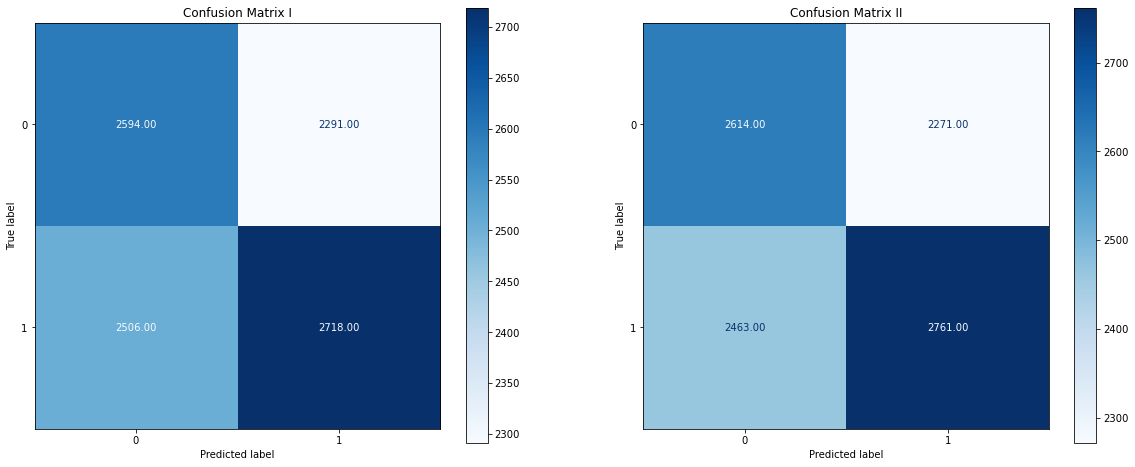
\includegraphics[width=1\textwidth]{ROC.png}}
	\caption{ROC curve}
\end{figure}

\begin{figure}[H]
	\centerline{\includegraphics[width=1\textwidth]{confusion\_matrix.png}}
	\caption{Confusion Matrix}
\end{figure}

\begin{table}[htbp]
	\centering
	\begin{tabular}{lrrrrrr}
		\toprule
		Test    & max\_depth & min\_samples\_split & MSE        & RMSE       & R2Train    & R2Test     \\
		\midrule
		Test I  & 5          & 6                   & 0.47452765 & 0.68885967 & 0.56024931 & 0.52547235 \\
		Test II & 1          & 2                   & 0.46829558 & 0.68432125 & 0.54570637 & 0.53170442 \\
		\bottomrule
	\end{tabular}
	\setlength{\abovecaptionskip}{0.3cm}
	\setlength{\belowcaptionskip}{0cm}

	\caption{Splits Test Result}
\end{table}

The results show that by adjusting max\_depth, min\_samples\_split, MSE can be reduced and R2 Score can be improved. More infomation can be accessed by '7. plots.ipynb'.

\section*{Question 3. Ensemble Learning}

Tree boosting is highly effective and widely used machine learning method. XGBoost stands for “Extreme Gradient Boosting”, where the term “Gradient Boosting” originates from the paper Greedy Function Approximation: A Gradient Boosting Machine, by Friedman. LightGBM (Light Gradient Boosting Machine) is a gradient boosting framework that uses tree based learning algorithms. In this experiment, we will use LGBMClassifier from LightGBM library to predict future prices of BTCUSDT by creating a custom list of features from the raw price series.

\subsection*{1. Retrieve Data}

\begin{figure}[H]
	\centerline{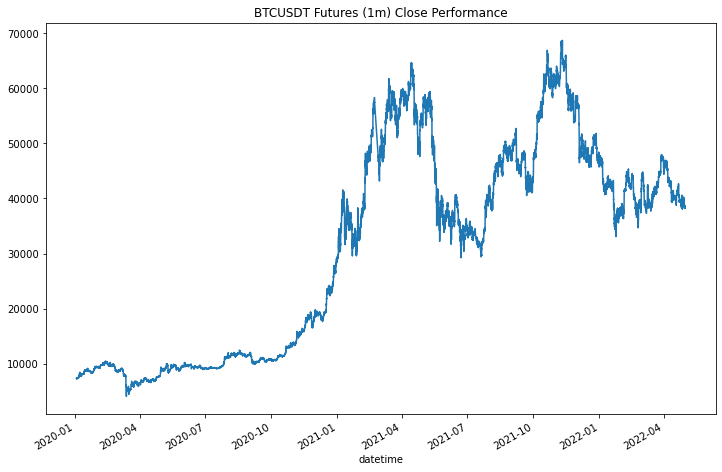
\includegraphics[width=1\textwidth]{Q3_Close_Performance.png}}
	\caption{BTCUSDT Close Price Performance}
\end{figure}

\subsection*{2. Factor Engineering}

Factors include: 'O-C', 'H-L', 'PR5', 'PR10', 'PR20', 'PR30', 'PR60', 'MOM5', 'MOM10', 'MOM20', MOM30', 'MOM60', 'SMA5', 'SMA10', 'SMA20', 'SMA30', 'SMA60', and 'EMA'. 'Sign' is designed as the label with ratio 1.0.

\begin{equation}
	y_t= \left\{
	\begin{aligned}
		+1 & , if\ p_{t+1} > 1.0 * p_t  \\
		0  & , if\ p_{t+1}\ \ otherwise \\
	\end{aligned}
	\right\}
\end{equation}

\begin{figure}[H]
	\centerline{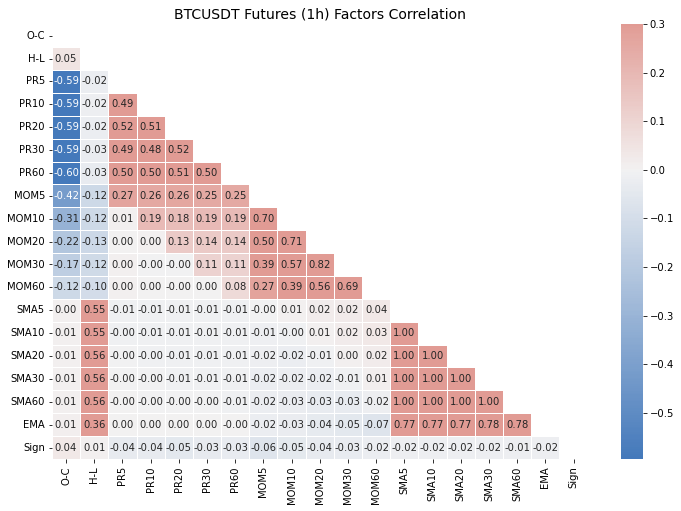
\includegraphics[width=1\textwidth]{Q3_Corr.png}}
	\caption{BTCUSDT Factors Correlation}
\end{figure}

\subsection*{3. Hyperparameters Tuning and Pruned}

We use MinMaxScaler as the model's scaler, TimeSeriesSplit to split the data and RandomizedSearchCV to tune and prune parameters: learning\_rate, max\_depth, min\_child\_weight, num\_leaves and colsample\_bytree. The scoring is f1. To improve computing efficiency, we use GPU to accelerate the progress.

After 5 minutes of computing, we get the optimal parameters: 'num\_leaves': 10, 'min\_child\_weight': 3, 'max\_depth': 5, 'learning\_rate': 0.25, 'colsample\_bytree': 0.5, and the best\_score\_ is: 0.5822.

\subsection*{4. Prediction}

Through the trained model, we get prediction results: mse: 0.4922, rmse is 0.7016, r2train is 0.7195, r2test is 0.5078. The following are Confusion Matrix, ROC Curve, Factors Importance and Tree Digraph. For more information, please refer to '8. XGBoost.ipynb'.

\begin{figure}[H]
	\centerline{\includegraphics[width=0.7\textwidth]{Q3\_Confusion\_Matrix.png}}
	\caption{Confusion Matrix}
\end{figure}

\begin{figure}[H]
	\centerline{\includegraphics[width=0.7\textwidth]{Q3\_ROC.png}}
	\caption{ROC Curve}
\end{figure}

\begin{figure}[H]
	\centerline{\includegraphics[width=0.7\textwidth]{Q3\_Importance.png}}
	\caption{Factors Importance}
\end{figure}

\begin{figure}[H]
	\centerline{\includegraphics[width=1\textwidth]{Q3\_Tree.png}}
	\caption{Tree Digraph}
\end{figure}

\section*{Question 4. Basktesting \& Kelly}

This experiment is divided into two parts. One is backtesting (100\% bets), and another is Kelly optimal basktesting. Kelly allocation to the asset computed with probability $p$ taken from predict\_proba() is $2p-1$. From the results, we find that most of indicators become worse after using Kelly allocation. Annual Return decreses from -2.295\% to -17.99\%, Sharpe ratio becomes deeper than before, and Max drawdown decreases from -64.212\% to -99.965\%. The good news is that Annual volatility and Daily value at risk become better. The code is in the file: '9. Backtesting \& Kelly.ipynb'. Maybe Kelly allocation reduces the gain, which results in increased great losses.

\begin{figure}[H]
	\centering
	\begin{minipage}[t]{0.4\textwidth}
		\centering
		\centerline{\includegraphics[width=0.8\textwidth]{Q3\_Backtesting.png}}
		\caption{BackTesting}
	\end{minipage}
	\hfill
	\begin{minipage}[t]{0.4\textwidth}
		\centering
		\centerline{\includegraphics[width=0.8\textwidth]{Q3\_Backtesting\_Kelly.png}}
		\caption{Kelly BackTesting}
	\end{minipage}
\end{figure}

\begin{figure}[H]
	\centerline{\includegraphics[width=0.8\textwidth]{Q3\_CumReturns.png}}
	\caption{Back Testing Digraph}
\end{figure}

\begin{figure}[H]
	\centerline{\includegraphics[width=0.9\textwidth]{Q3\_CumReturns\_Kelly.png}}
	\caption{Kelly Back Testing Digraph}
\end{figure}

\end{document}